%Part of/Parte di https://github.com/f-dinucci/appuntiMeccanicaFluidi/
%License/Licenza Creative Commons Attribution-ShareAlike 4.0 International (CC BY-SA 4.0) - attribution/attribuzione Francesco Di Nucci
%See also/Vedere anche https://creativecommons.org/licenses/by-sa/4.0/ and/e https://creativecommons.org/licenses/by-sa/4.0/legalcode
%
\chapter{Appendice B: Cassetta degli attrezzi}

%SUBSECTION
\subsection*{Derivata composta}
Derivata composta di funzioni di più variabili:
	\begin{equation*}
		\begin{gathered}
			\dv{f}{x} = \pdv{\lambda} f(x(\lambda), y(\lambda), z(\lambda), t(\lambda)) = \\
			= \pdv{f}{x} \dv{x}{\lambda} + \pdv{f}{y} \dv{y}{\lambda} + \pdv{f}{z} \dv{z}{\lambda} + \pdv{f}{t} \dv{t}{\lambda}\\
			\text{se $\lambda = t \rightarrow \dv{t}{\lambda} = 1$}\\
			\dv{f}{t} = \pdv{f}{x} \dv{x}{t} + \pdv{f}{y} \dv{y}{ta} + \pdv{f}{z} \dv{z}{t} + \pdv{f}{t}
		\end{gathered}
	\end{equation*}

%SUBSECTION
\subsection*{Derivata sostanziale}
Per una qualsiasi funzione $f$ si può introdurre la derivata sostanziale, che rappresenta le variazioni dal punto di vista di un osservatore in moto con il fluido (cioè quando la derivata della traiettoria coincide con la velocità):
	\begin{equation*}
		\begin{gathered}
			\pdv{f}{t} + \uline{v} \vdot \grad{f} \equiv \frac{\mathrm{D} f}{\mathrm{D} t}\\
			\frac{\mathrm{D} f}{\mathrm{D} t} = \pdv{f}{t} + v_1 \pdv{f}{x_1} + v_2 \pdv{f}{x_2} + v_3 \pdv{f}{x_3} = \pdv{f}{t} + \uline{v} \vdot \grad{f}
		\end{gathered}
	\end{equation*}
È detta sostanziale dato che segue una particella di ``sostanza`` nel moto.

%SUBSECTION
\subsection*{Formula di Gauss e Teorema della divergenza}
Richiamo utile per passare da un integrale di volume ad uno di superficie.

Secondo la formula di Gauss:
	\begin{equation*}
		\begin{gathered}
			\int \pdv{f}{x_i} \dd{V} = \oint {f n_i \dd{S}}\\
			\text{alias}\\
			\int_V \grad{f} \dd{V} = \oint_{\partial V} f \uline{n} \dd{S}
		\end{gathered}
	\end{equation*}
	
Questa è una sorta di formula generale (che vale anche per i singoli termini) dalla quale deriva il teorema della divergenza:
	\begin{equation*}
		\int{ \left( \pdv{v_1}{x_1} + \pdv{v_2}{x_2} + \pdv{v_3}{x_3} \right) \dd{V}} = \oint{ \left( v_1 n_1 + v_2 n_2 + v_3 n_3 \right) \dd{S}} 
	\end{equation*}

In termini impropri è come se si facesse un'operazione del tipo (utilizzando la formula fondamentale del calcolo integrale):
	\begin{equation*}
		\int{\pdv{f}{x_1} \dd{x_1} \dd{x_2} \dd{x_3}} = \int{f \dd{x_2} \dd{x_3}}
	\end{equation*}
	
Per vettori e tensori:
	\begin{equation*}
		\begin{gathered}
			\int \div{\uline{f}} \dd{V} = \oint \uline{n} \vdot \uline{f} \dd{S}\\
			\int \div{\uuline{f}} \dd{V} = \oint_{\partial V} \uline{n} \vdot \uuline{f} \dd{S}\\
		\end{gathered}
	\end{equation*}
	
Ricordare che l'ordine dei fattori è importante (salvo in caso di tensori simmetrici).

%SUBSECTION
\subsection*{Formula di Leibnitz}
Si parte dal problema monodimensionale:
	\begin{equation*}
		\dv{t} \int_{a(t)}^{b(t)} f \dd{x} = ?
	\end{equation*}
	\begin{figure}[H]
		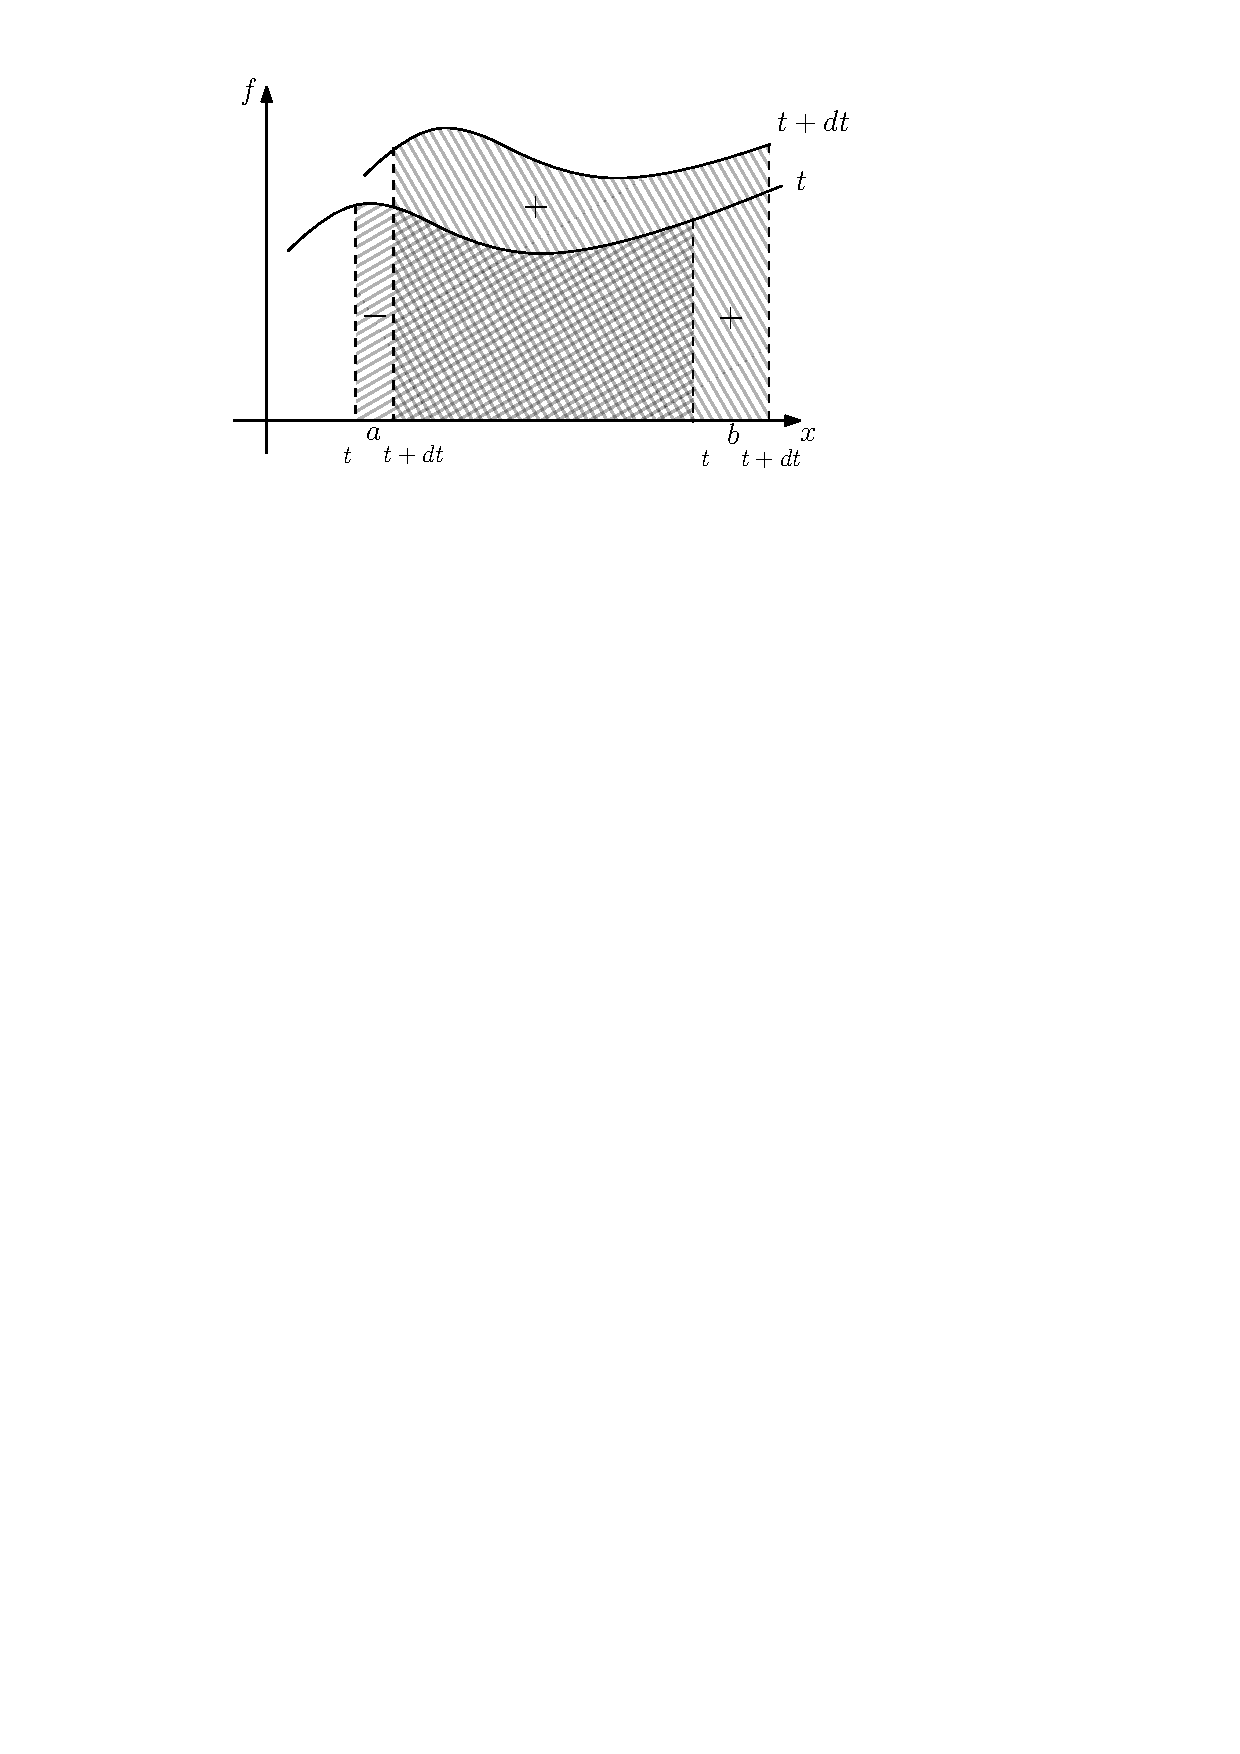
\includegraphics[scale=0.6]{./Appendice B - Cassetta degli attrezzi/B.1}
		\centering
		\caption{Si vede l'integrale come area del rettangoloide}
	\end{figure}
Dato che la curva e gli estremi si spostano al variare del tempo, al limite conta solamente quello che accade nei tre ``pezzi'' al contorno:
	\begin{equation*}
		\begin{gathered}
			\int_{a(t+dt)}^{b(t+dt)} f(t+dt, x) \dd{x} = \\
			= \int_{a(t)}^{b(t)} f(t, x) \dd{x} + \dd{t} \int_a^b \pdv{f}{t} \dd{x} + \dd{t} \dv{b}{t} f(t, b) - \dd{t} \dv{a}{t} f(t,a) \\
		\end{gathered}
	\end{equation*}			
Quindi dividendo per $\dd{t}$:
	\begin{equation*}			
		\dv{t} \int_a^b f \dd{x} = \int_a^b \pdv{f}{t} \dd{x} + \dv{b}{t} f(t,b) - \dv{a}{t} f(t,a)  \quad \textbf{(Formula di Leibnitz)}
	\end{equation*}

%SUBSECTION
\subsection*{Gradiente}
Il gradiente di un vettore $\uline{v}$ è:
	\begin{equation*}
			\grad{\uline{v}} = 
				\begin{bmatrix} 
					\pdv{x_1} & \pdv{x_2} & \pdv{x_3}
				\end{bmatrix}
				\begin{bmatrix} 
					v_1 & v_2 & v_3
				\end{bmatrix} 
					=
				\begin{bmatrix}
					\pdv{v_1}{x_1} & \pdv{v_1}{x_2} & \pdv{v_1}{x_3}\\
					\pdv{v_2}{x_1} & \pdv{v_2}{x_2} & \pdv{v_2}{x_3}\\
					\pdv{v_3}{x_1} & \pdv{v_3}{x_2} & \pdv{v_3}{x_3}\\
				\end{bmatrix}
	\end{equation*}


%SUBSECTION
\subsection*{Notazione di Einstein}
Per sottintendere una sommatoria si può utilizzare la notazione di Einstein:
	\begin{equation*}
		\uline{J}_M \vdot \uline{n} = J_{M1} n_1 + J_{M2} n_2 + J_{M3} n_3 = \sum_{j=1}^{3} {J_{Mj} n_j} = J_{Mj} n_j
	\end{equation*}

%SUBSECTION
\subsubsection*{Teorema del trasporto di Reynolds}
Analogo bi/tridimensionale della formula di Leibnitz.
Nel problema bidimensionale (analogo ragionamento si può estendere in 3D):
	\begin{equation*}
		\dv{t} \int_{S(t)} f(t, \uline{x}) \dd{S} = ?
	\end{equation*}
	\begin{figure}[H]
		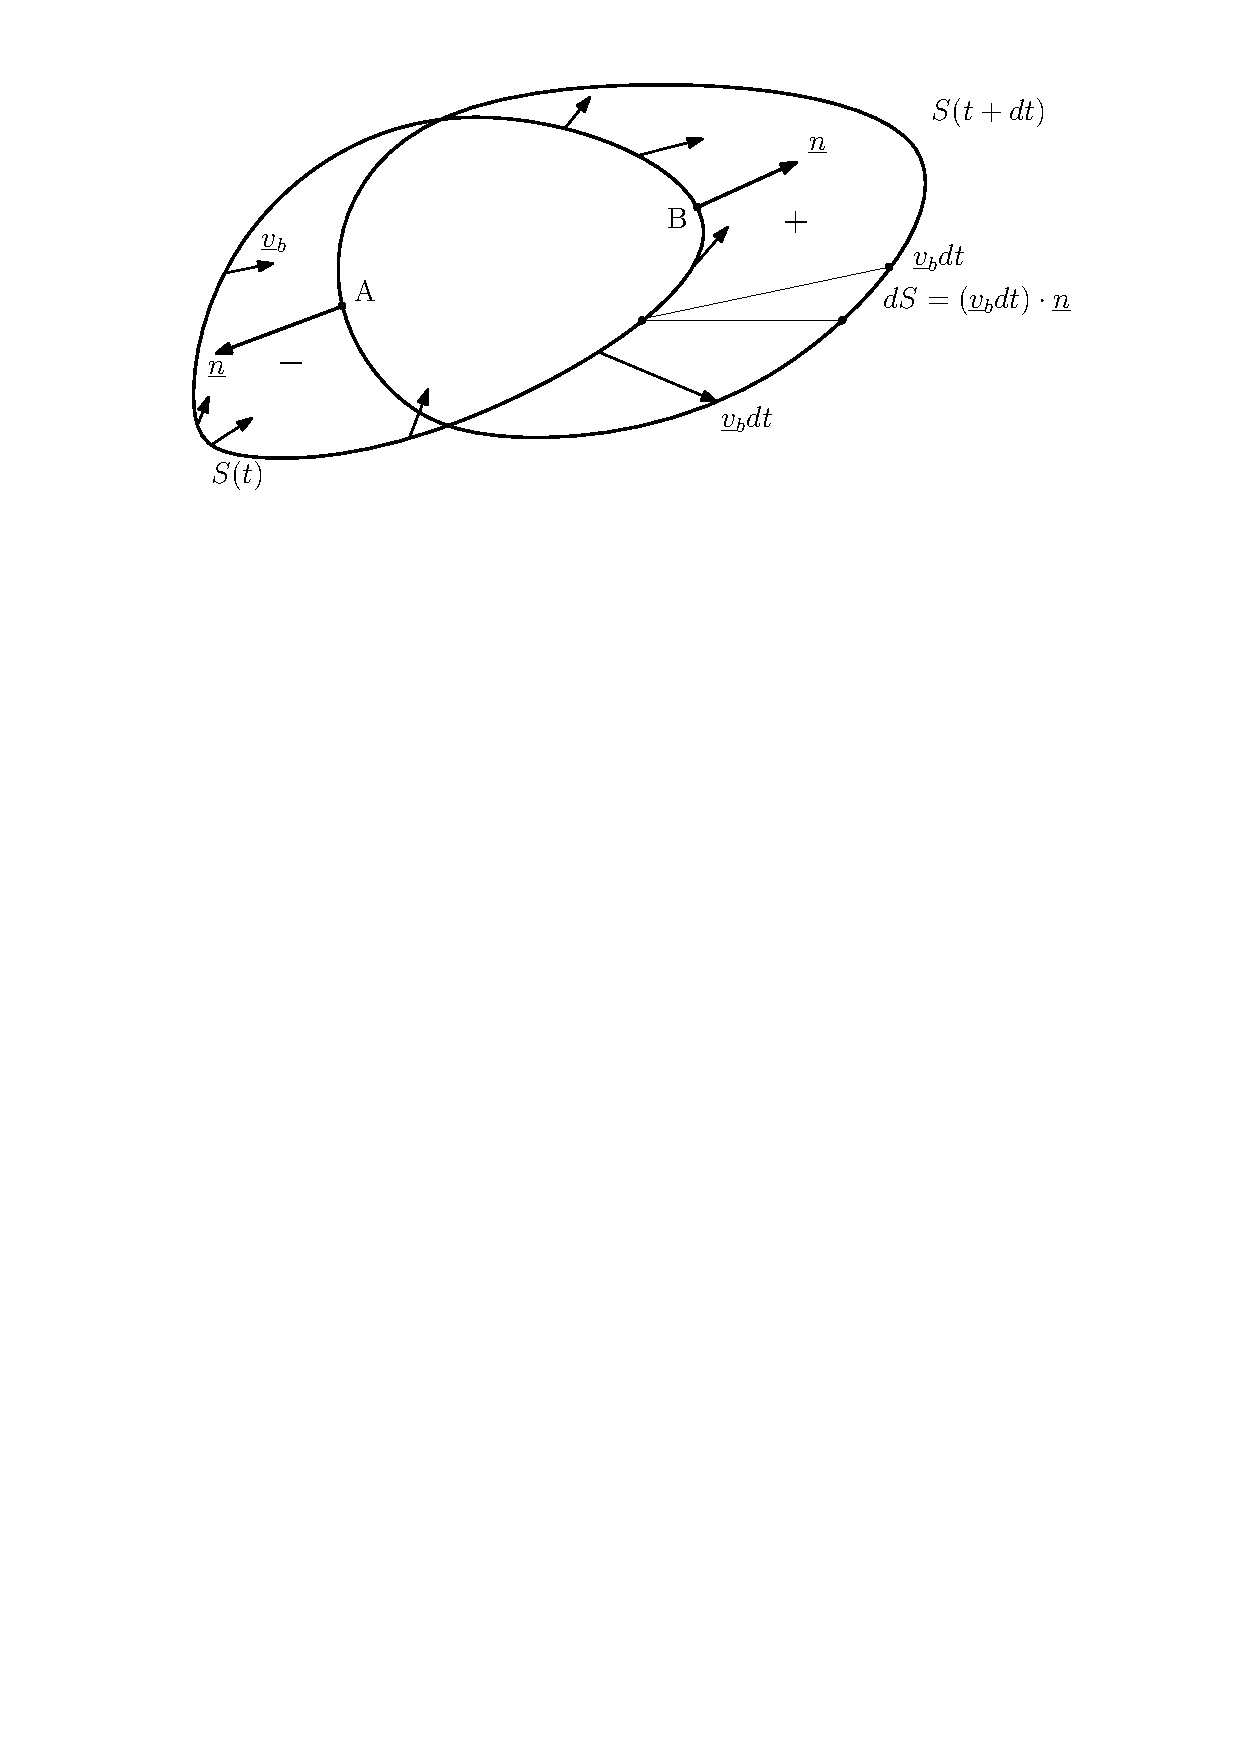
\includegraphics[scale=0.65]{./Appendice B - Cassetta degli attrezzi/B.2}
		\centering
		\caption{Si consideri cosa accade per un $\dd{t}$ infinitesimo}
	\end{figure}
Più $\dd{t}$ diminuisce, più la superficie varia di un infinitesimo, si caratterizza il movimento della superficie $S$ tramite una velocità $v_b$\footnote{Boundary velocity} associata ad ogni punto del contorno (un vettore per ogni punto).

Ogni punto del contorno si sposta di $\uline{v}_b \dd{t}$, si integra quindi l'area della "mezzaluna" avendo lo spostamento e la sua proiezione sulla normale:
	\begin{equation*}
		\begin{gathered}
			\int_{S(t+\dd{t})} f (t + \dd{t}, x) \dd{S} = \\
			= \int_{S(t)} f (t, \uline{x}) + \dd{t} \int \pdv{f}{t} \dd{S} + \dd{t} \int_{B} f \uline{v}_b \vdot \uline{n} \dd{c} - \dd{t} \int_A f \uline{v}_b \vdot \uline{n} \dd{c} \footnote{il segno di questo integrale cambia per via della discordanza con la normale} \\
			\text{quindi rispettivamente in due e tre dimensioni} \\
			\dv{t}  \int_{S(t)} f \dd{S} = \int \pdv{f}{t} \dd{S} + \oint f \uline{v}_b \vdot \uline{n} \dd{c}\\
			\dv{t} \int_{V(t)} f \dd{V} = \int \pdv{f}{t} \dd{V} + \oint f \uline{v}_b \vdot \uline{n} \dd{S}\\
		\end{gathered}
	\end{equation*}
I segni sono dovuti alla concordanza/discordanza nel prodotto scalare tra i versi di $\uline{v}_b$ e della normale $\uline{n}$ (che per convenzione è positiva verso l'esterno), il risultato della somma è tutto il contorno $c$.
